% --------------------------------------------------------------------------------
\newpage
\section{Echoic Memory Module}
% --------------------------------------------------------------------------------

% Make general target
\hypertarget{Concepts:EchoicMemoryModule}{}

% Make target for following functions:
\hypertarget{Concepts:IPEMLeakyIntegration}{}

\subsection{Introductory description}
% --------------------------------------------------------------------------------

An echo can be defined as a leaky integration with a given half
decay time. At each moment in time, a leaky integrator adds the
incoming signal value to an attenuated version of the previously
calculated value to form the newly calculated value. The half
decay time specifies the time it takes for an impulse signal to
reach half its original value.

The Echoic Memory Module (EMM) takes an image as input and gives
the leaky integrated image as output. The images are integrated so
that at each time step, the new image is calculated by taking a
certain amount of the old image which is then added with the new
incoming image.

The Echoic Memory Module can be applied to pitch completion
images, for example. We then start from our familiar APM, followed
by PCM, and apply EMM. The echo which we specify defines the
amount of context which we take into account. With very little (or
almost no) context we speak about \emph{local pitch images}. When
context is taken into account we use a longer half decay time and
call the images \emph{global pitch images}. EMM has been used in
\citeA{article:MusicPerception:Leman:2000} to construct the
pitch images of an echoic memory. In our global chart of image
transformation modules EMM is localized in the middle part
(perception section) of figure \ref{Fig:ModulesEMM}. The
application is described in detail in the chapter on
\hyperlink{Concepts:IPEMGenerateProbes}{{tonality induction
experiments}}.
\begin{figure}[h]
    \centering
    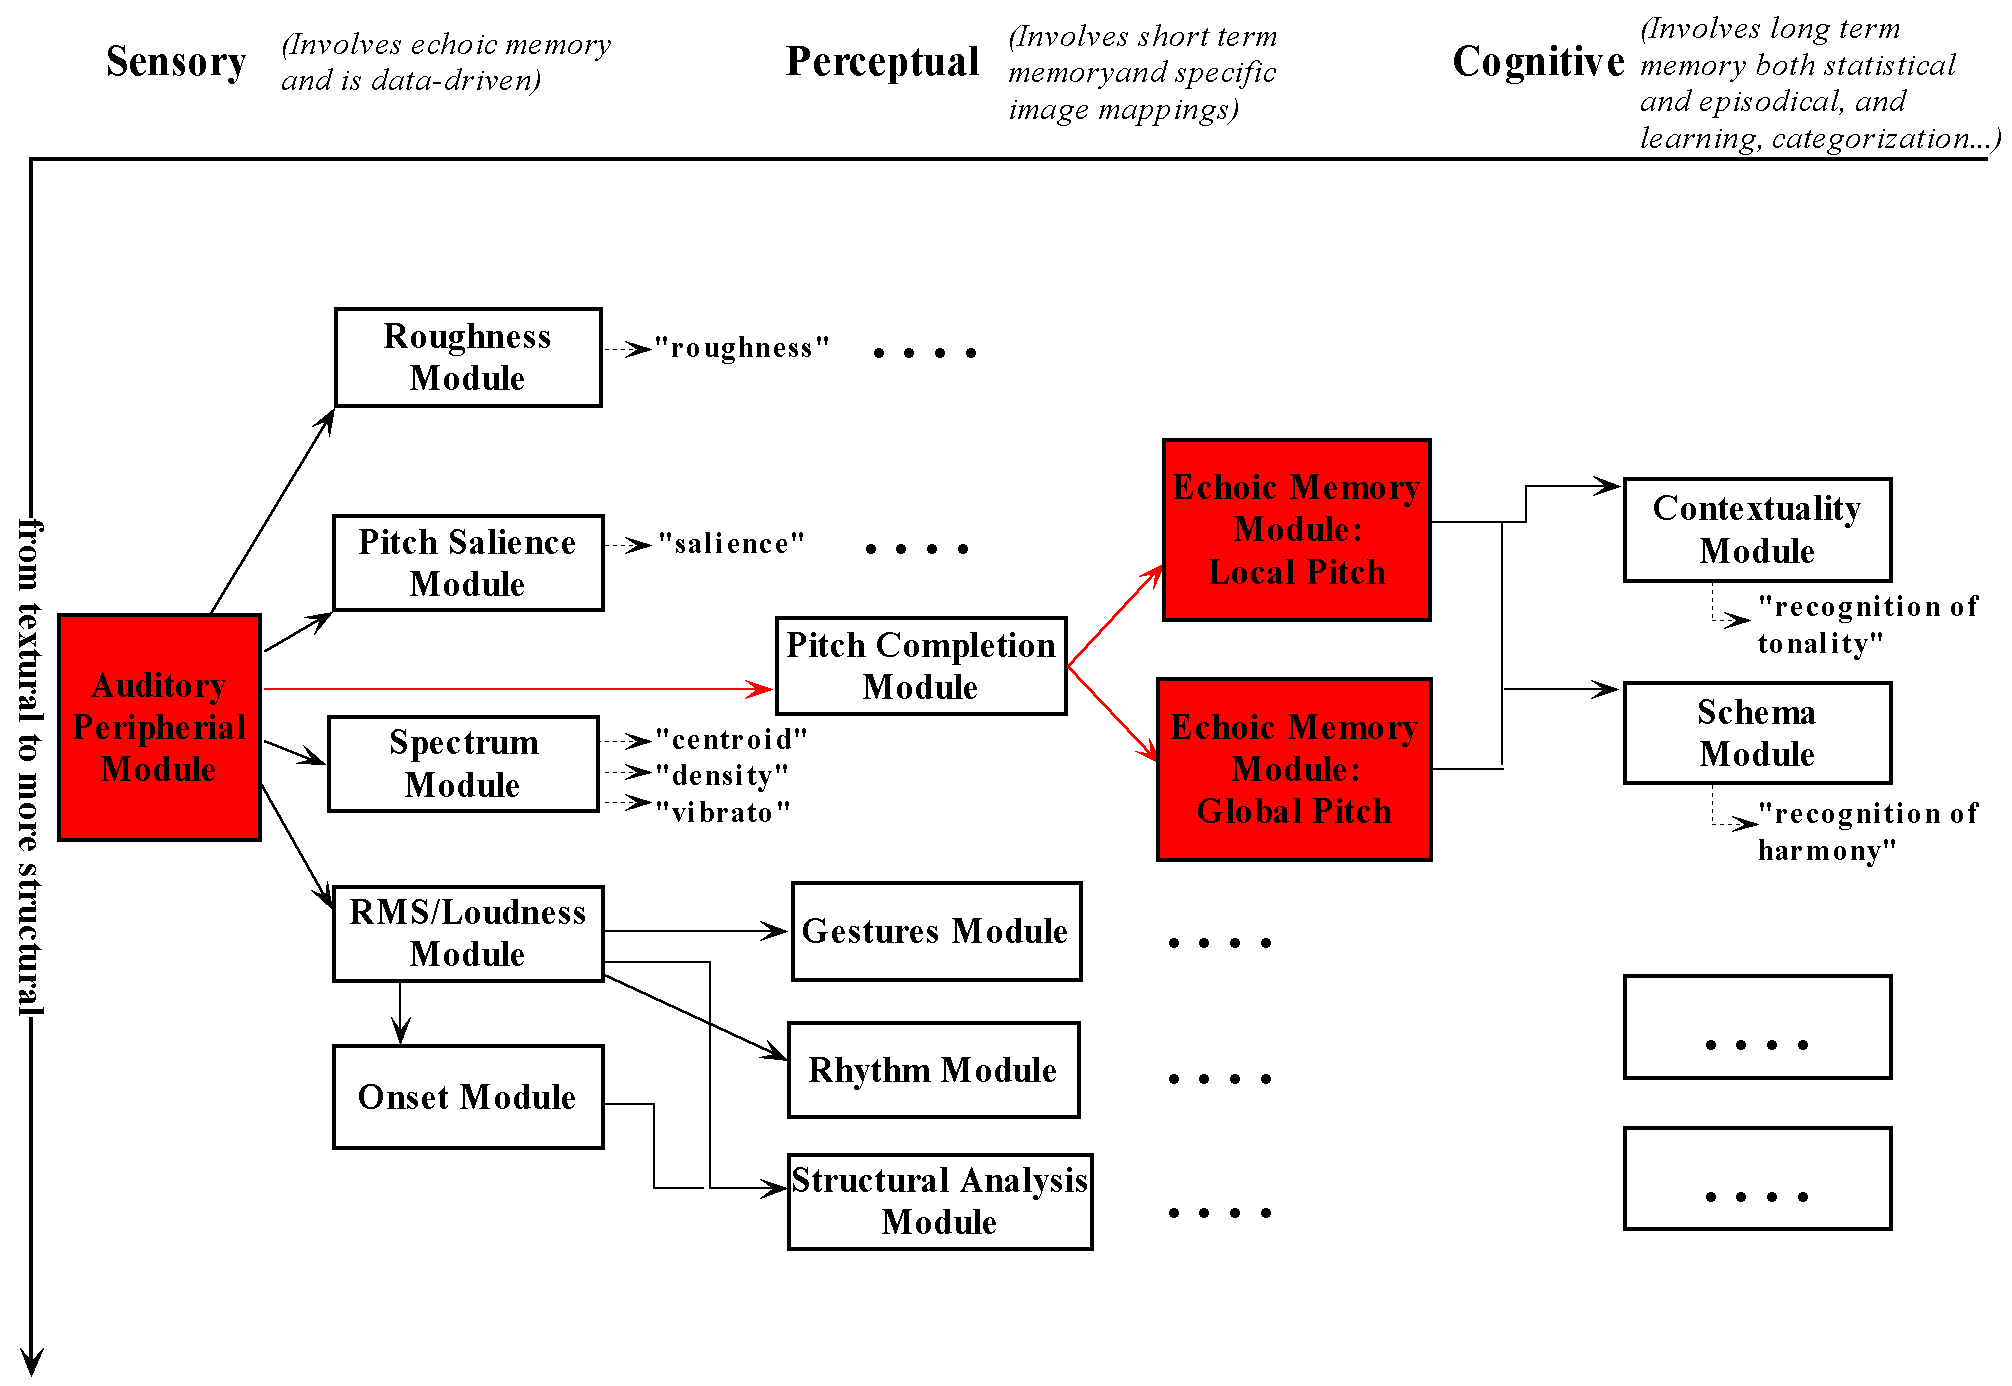
\includegraphics[width=\textwidth]{Graphics/ModulesEMM}
    \caption{Chart of image transformation modules, with EMM highlighted}
    \label{Fig:ModulesEMM}
\end{figure}
Figure \ref {Fig:EMMModule} shows the modules involved in the
image transformation process.
\begin{figure}[h]
    \centering
    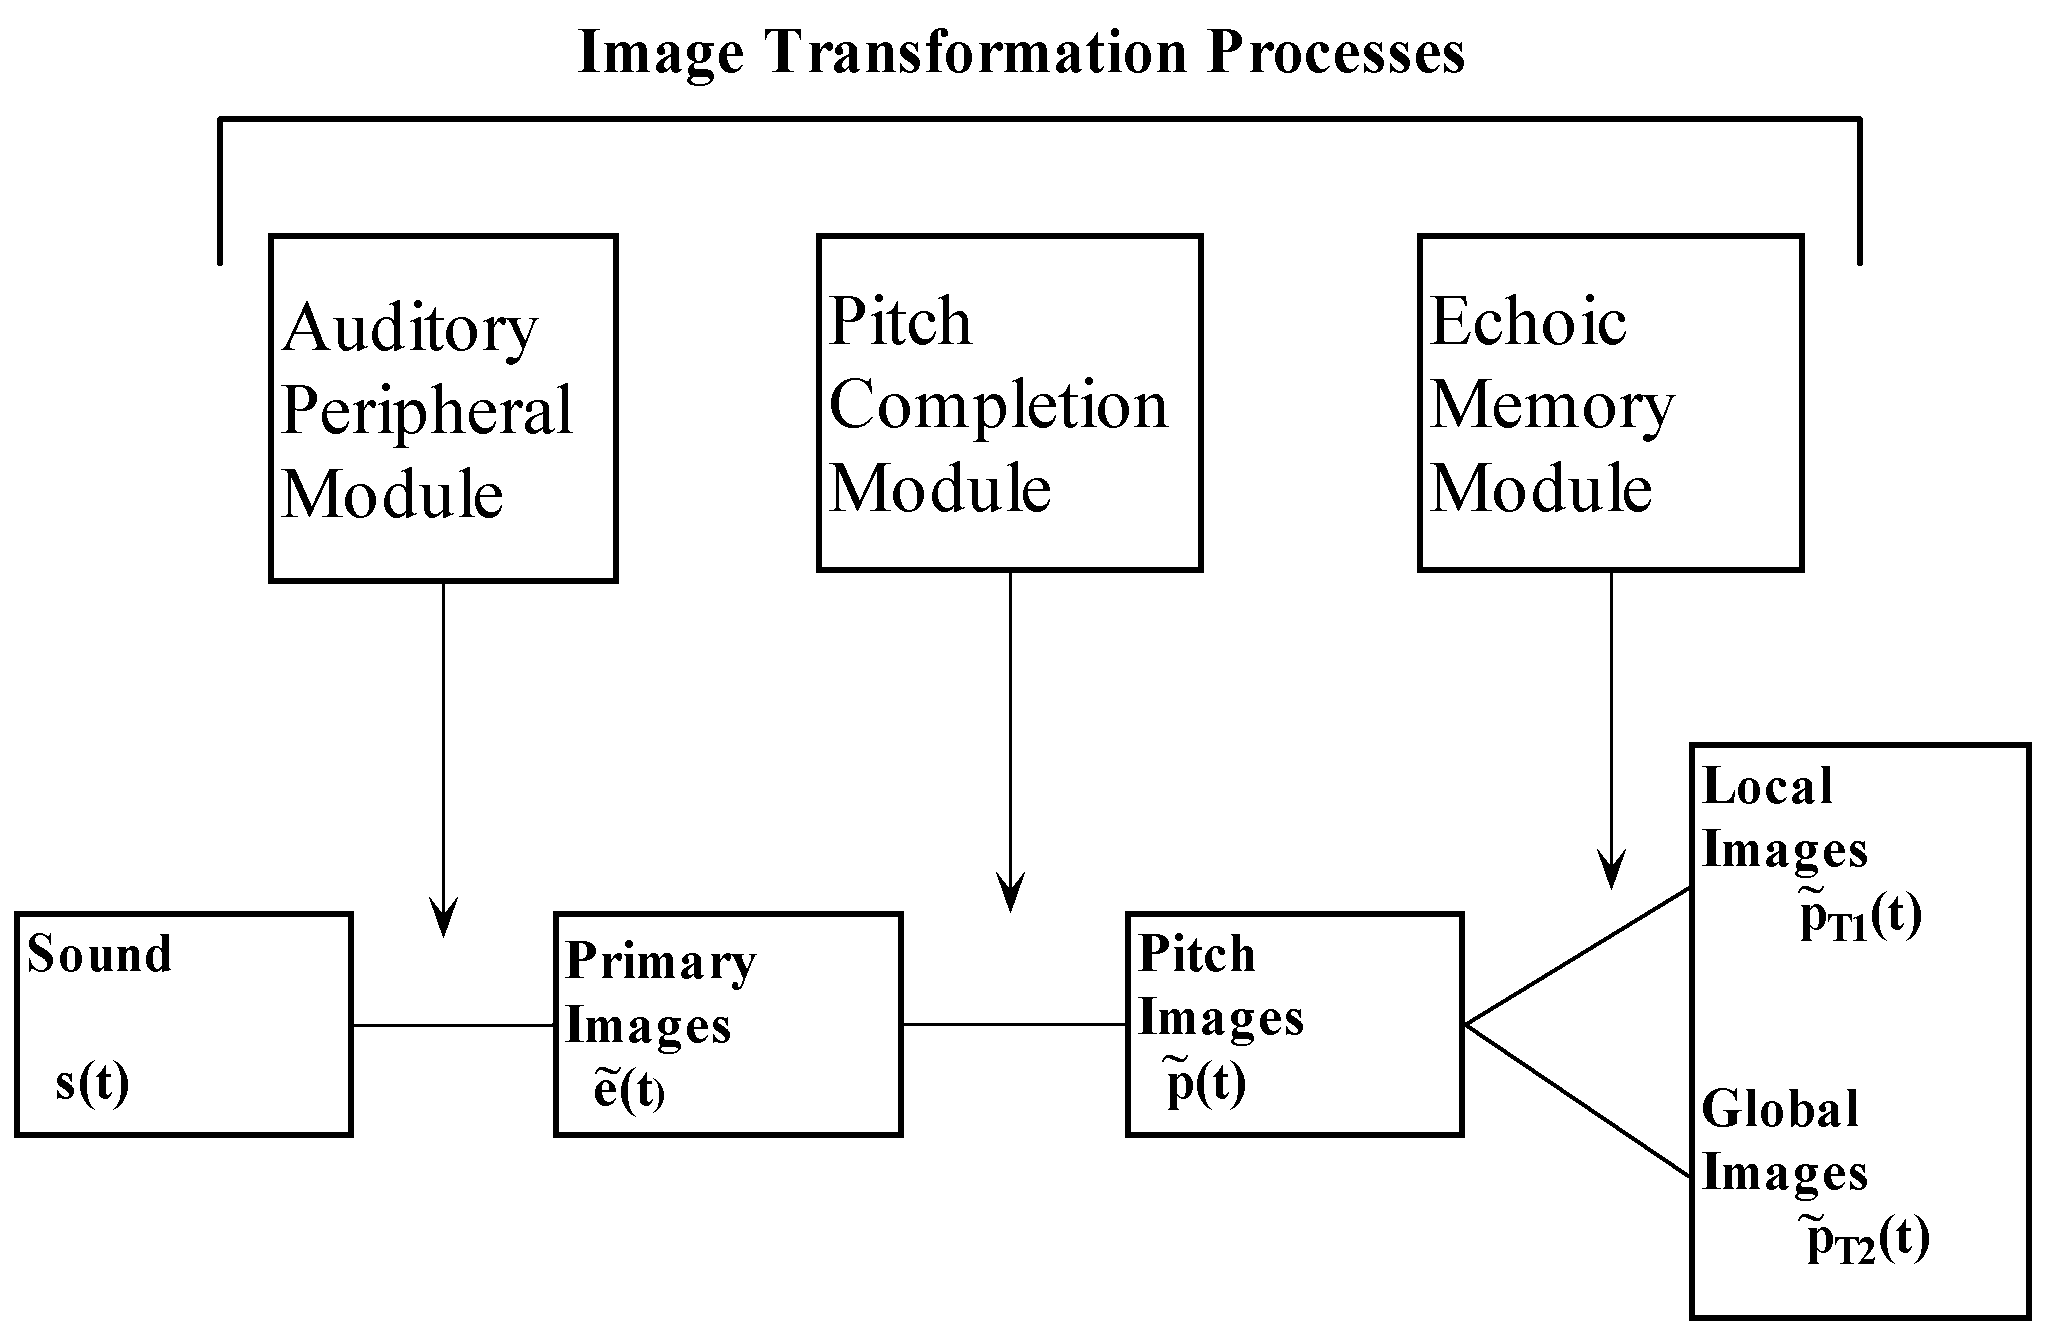
\includegraphics[width=\IPEMDefaultFigureWidth]{Graphics/EMMModule}
    \caption{Image Transformation Process: Echoic Memory Module}
    \label{Fig:EMMModule}
\end{figure}

\subsection{Functional-logical description}
% --------------------------------------------------------------------------------

A symbolic representation of the Echoic Memory Module may be written as:
\begin{equation}
EMM: \tilde{p}(t) \rightarrow \tilde{p}_T(t)
\end{equation}
where $T$ denotes the {\sl echo} in seconds, $\tilde{p}(t)$
denotes a pitch completion image and $ \tilde{p}_T(t)$ an echoed
image.


\subsection{Signal processing description}
% --------------------------------------------------------------------------------

$\tilde{p}_T(0) = \tilde{p}(0)$

$\tilde{p}_T(t) = \tilde{p}(t) ~+~
\tilde{p}_T(t-1)*2^{\frac{-1}{T}}$ \quad , $t \neq 0$


\subsection{Implementation}
% --------------------------------------------------------------------------------

\begin{tabularx}{\linewidth}{llX}
\hyperlink{FuncRef:IPEMLeakyIntegration}{IPEMLeakyIntegration} & - & Calculates leaky integration with specified half decay time\\
\end{tabularx}


\subsection{Examples}
% --------------------------------------------------------------------------------

The Echoic Memory Module can be applied to a pitch completion
image to obtain a local and a global pitch image. A local pitch
image can be defined as $\tilde{p}_{T=0.1}(t)$, with an echo of
0.1 s, while a global pitch image can be defined as
$\tilde{p}_{T=1.5}(t)$, with the echo of 1.5 s. Local images are
built up by echoes which, by definition, are smaller than echoes
for the global images. Use the following MATLAB functions to
create those pitch images:\\

\begin{IPEMCodeEnvironment}
[ANI,ANIFreq,ANIFilterFreqs] = IPEMCalcANIFromFile('SchumannKurioseGeschichte.wav');
\newline [PP,PPFreq,PPPeriods,PPFANI] = IPEMPeriodicityPitch(ANI,ANIFreq);
\newline LocalIntegration = IPEMLeakyIntegration(PP,PPFreq,0.1,0.1,1);
\newline GlobalIntegration = IPEMLeakyIntegration(PP,PPFreq,1.5,1.5,1);
\end{IPEMCodeEnvironment}\\

Figure \ref{Fig:EMMPitchImages} shows the pitch images for the
\IPEMSound{Sounds/SchumannKurioseGeschichte.wav}{excerpt of
Schumann's Kuriose Geschichte}.

\begin{figure}[h]
    \centering
    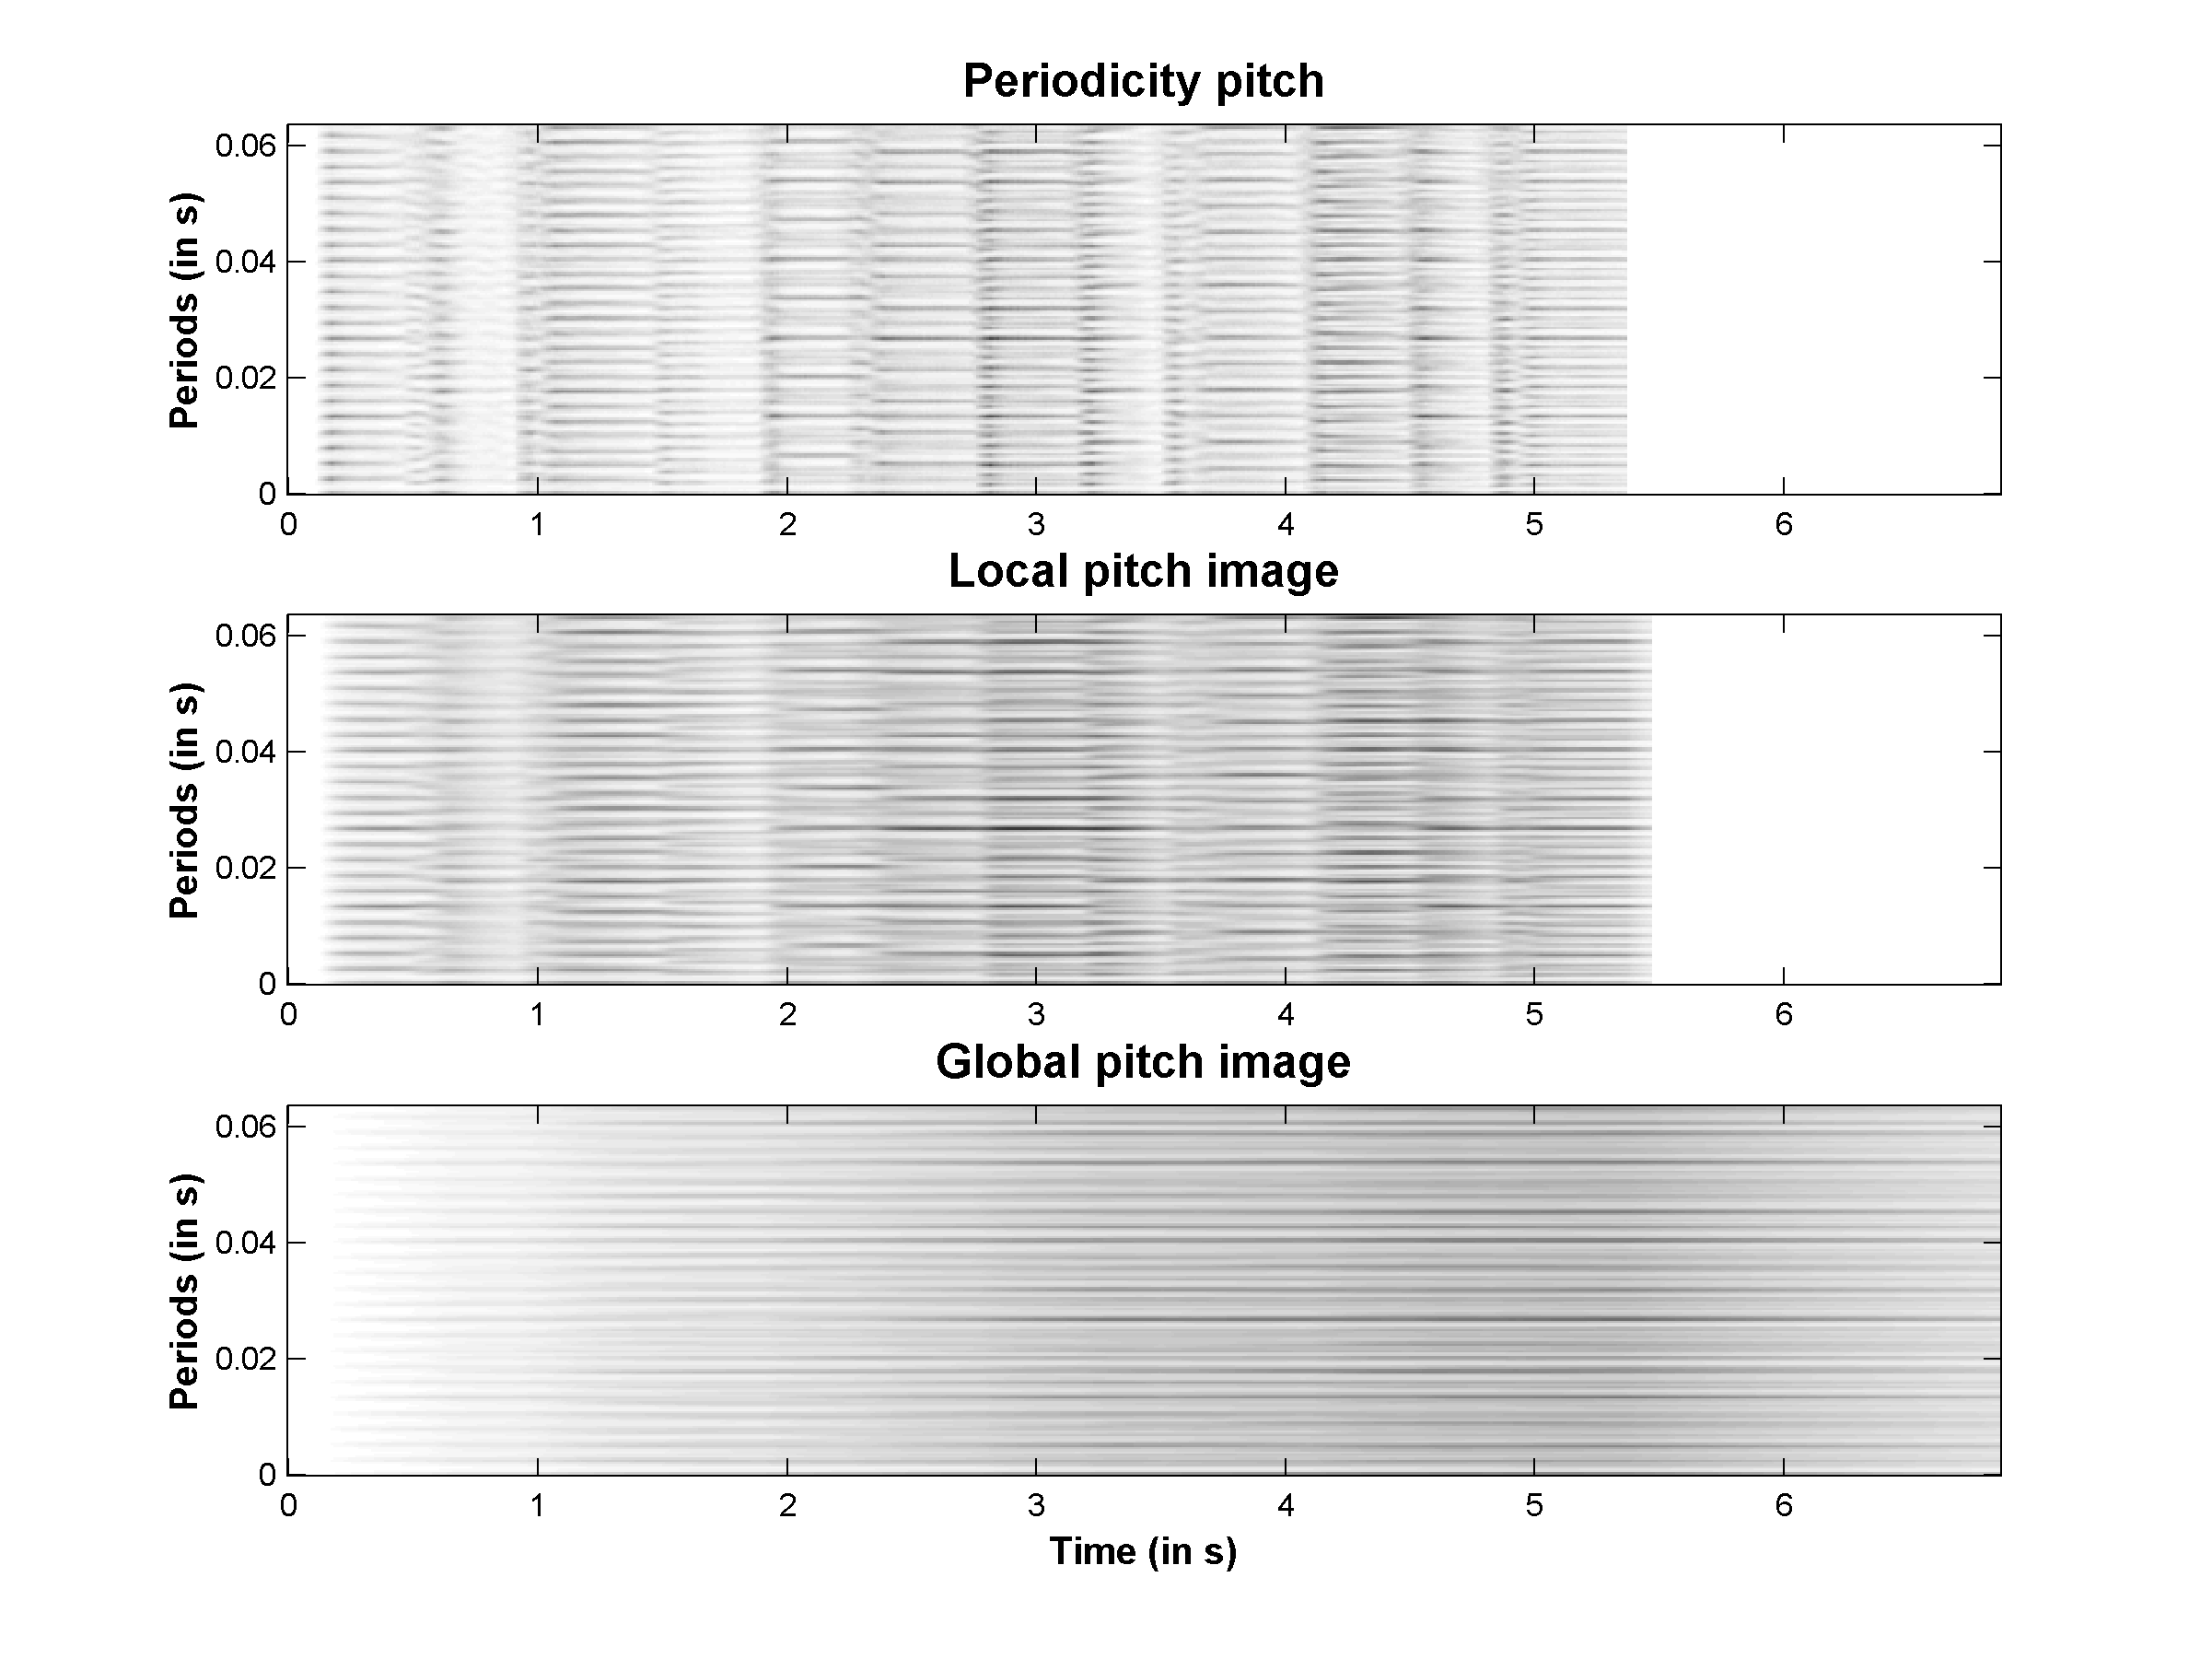
\includegraphics[width=\IPEMDefaultFigureWidth]{Graphics/EMMPitchImages}
    \caption{Top: periodicity pitch for the excerpt of Schumann's Kuriose Geschichte
    Middle: local pitch image of Schumann's Kuriose Geschichte (echo of 0.1 s).
    Bottom: global pitch image (echo of 1.5 s)}
    \label{Fig:EMMPitchImages}
\end{figure}
